\subsection{Robot System Controller}
The robot is controlled using the schematic shown in Figure \ref{fig:control_schematic}, referred to as the "system controller". This should not be confused with the "robot controller" which refers to the controller that maps target motions to joint values. 

\begin{figure}[h]
    \centering
    \makebox[\textwidth][c]{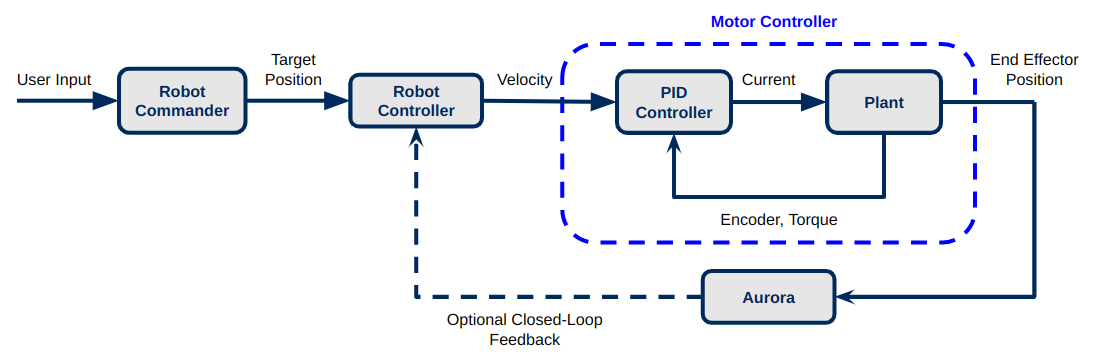
\includegraphics[width=\textwidth]{images/control_schematic.png}}
    \caption{Robot system controller schematic}
    \label{fig:control_schematic}
\end{figure}

\subsubsection{Controller Description}
\paragraph{A high level commander} module maintains the robot's state at all times. This module interfaces with the robot user, and determines which operation modes the robot is in. It handles logging, recovery behaviour, and manages a watchdog thread for each component of the system that will raise an error if any process dies. All robot states are described in Table \ref{tab:controller_states}. During states that are engaged in point tracking, a termination criteria of the end effector being within \SI{2}{cm} of the goal point is used. During trajectory tracking, no such condition is required as the goal point is progressed in time using a predefined trajectory. This module is referred to as the robot commander. 

\paragraph{A closed loop cascade controller} controls the motion of the robot. The inner loop uses a PID controller in conjunction with motor encoder feedback and a reference signal from the robot controller to determine the current to be sent to each motor. The gains used in this controller are shown in Table \ref{tab:motor_controller_gains}. This loop is referred to as the motor controller. 

\begin{table}[h]
    \centering
    \caption{Motor controller gains}
    \begin{tabular}{p{0.25\linewidth} | p{0.1\linewidth} | p{0.1\linewidth} | p{0.1\linewidth}}
        \textbf{Controller} & \textbf{$K_p$} & \textbf{$K_d$} & \textbf{$K_i$} \\
        \hline
        Position & 20 & 0.2 & 10 \\
        Position (Recovery) & 0.05 & 0.7 & 0.03 \\
        Velocity & 3 & 0 & 60 \\
    \end{tabular}
    \label{tab:motor_controller_gains}
\end{table}

\paragraph{The robot controller} determine the joint displacements or joint rates required to achieve a desired end effector motion. With this setup, the controller can either operate in a closed-loop scenario using measurements from the Aurora tracking system, or in an open-loop scenario, where an external state-estimation pipeline must be implemented. Explicit state estimation of this robot is outside of the scope of this thesis, so each proposed baseline controller will operate in the closed-loop configuration. 

\begin{table}[p]
    \centering
    \caption{Controller state description}
    \makebox[\textwidth][c]{\begin{tabular}{p{0.2\linewidth} | p{0.4\linewidth} | p{0.35\linewidth} }
        \textbf{State} & \textbf{Description} & \textbf{Exit Condition} \\
        \hline
        ERROR & The robot has experienced a critical error & Manual reset of the software and hardware \\
        \hline
        STOPPED & The robot is blocked from tracking reference signals. Used when the robot should remain stationary while code runs & State moves to READY after code is completed \\
        \hline
        RANDOM TRACKING & The robot is tracking random target points. Used during data collection & User terminated \\
        \hline
        REFERENCE TRACKING & The robot is tracking a pre-loaded reference trajectory. Used during model testing & Returns to READY when reference trajectory is complete  \\
        \hline
        REFERENCE STARTING & The robot is moving towards the start of a provided reference trajectory & Moves to HOLDING once the robot reaches the starting point to a reference trajectory \\
        \hline
        MANUAL TRACKING JOINT & The robot is tracking a point determined through the user control API in joint space & User terminated \\
        \hline
        MANUAL TRACKING TASK & The robot is tracking a point determined through the user control API in task space & User terminated \\
        \hline
        RECOVER & The robot is recovering from a lost Aurora signal. It is returning to the home position & Moves to READY when home position is reached \\
        \hline
        READY & The robot is stationary and able to take new commands & User terminated \\  \hline
        HOLDING & The robot is intentionally waiting at a point before progressing to the next command. Used during testing to provide time to set up video feeds & Moves to REFERENCE TRACKING after a set period of time \\
        \hline
    \end{tabular}}
    \label{tab:controller_states}
\end{table}

\subsubsection{Lost AURORA Recovery}
In the case of lost AURORA measurements, a recovery mode is entered where the robot returns to its home position using only motor encoder feedback. The home position is where both arms are fully extended and the motor encoders read a rotation of \SI{0}{rad}. This recovery behaviour is the only motion that can be executed in a closed-loop configuration without AURORA measurements. 